\documentclass[a4paper]{book}
\usepackage{makeidx}
\usepackage{natbib}
\usepackage{graphicx}
\usepackage{multicol}
\usepackage{float}
\usepackage{listings}
\usepackage{color}
\usepackage{ifthen}
\usepackage[table]{xcolor}
\usepackage{textcomp}
\usepackage{alltt}
\usepackage{ifpdf}
\ifpdf
\usepackage[pdftex,
            pagebackref=true,
            colorlinks=true,
            linkcolor=blue,
            unicode
           ]{hyperref}
\else
\usepackage[ps2pdf,
            pagebackref=true,
            colorlinks=true,
            linkcolor=blue,
            unicode
           ]{hyperref}
\usepackage{pspicture}
\fi
\usepackage[utf8]{inputenc}
\usepackage{mathptmx}
\usepackage[scaled=.90]{helvet}
\usepackage{courier}
\usepackage{sectsty}
\usepackage[titles]{tocloft}
\usepackage{doxygen}
\lstset{language=C++,inputencoding=utf8,basicstyle=\footnotesize,breaklines=true,breakatwhitespace=true,tabsize=8,numbers=left }
\makeindex
\setcounter{tocdepth}{3}
\renewcommand{\footrulewidth}{0.4pt}
\renewcommand{\familydefault}{\sfdefault}
\hfuzz=15pt
\setlength{\emergencystretch}{15pt}
\hbadness=750
\tolerance=750
\begin{document}
\hypersetup{pageanchor=false,citecolor=blue}
\begin{titlepage}
\vspace*{7cm}
\begin{center}
{\Large \-My \-Project }\\
\vspace*{1cm}
{\large \-Generated by Doxygen 1.7.6.1}\\
\vspace*{0.5cm}
{\small Thu Apr 11 2013 08:45:05}\\
\end{center}
\end{titlepage}
\clearemptydoublepage
\pagenumbering{roman}
\tableofcontents
\clearemptydoublepage
\pagenumbering{arabic}
\hypersetup{pageanchor=true,citecolor=blue}
\chapter{\-C\-S\-C\-I 102 \-Homework \#4}
\label{index}\hypertarget{index}{}\hypertarget{index_purpose}{}\section{\-Purpose/\-Overview}\label{index_purpose}
\-P\-A4 puzzle game \-G\-U\-I implementation assignment 
\chapter{\-Class \-Index}
\section{\-Class \-Hierarchy}
\-This inheritance list is sorted roughly, but not completely, alphabetically\-:\begin{DoxyCompactList}
\item \contentsline{section}{\-Board}{\pageref{classBoard}}{}
\item \contentsline{section}{\-Board\-Less\-Than}{\pageref{structBoardLessThan}}{}
\item \contentsline{section}{\-My\-List$<$ \-T $>$}{\pageref{classMyList}}{}
\item \contentsline{section}{\-P\-M\-Min\-List}{\pageref{classPMMinList}}{}
\item \contentsline{section}{\-Puzzle\-Heuristic}{\pageref{classPuzzleHeuristic}}{}
\begin{DoxyCompactList}
\item \contentsline{section}{\-Manhattan\-Heuristic}{\pageref{classManhattanHeuristic}}{}
\item \contentsline{section}{\-Out\-Of\-Place\-Heuristic}{\pageref{classOutOfPlaceHeuristic}}{}
\end{DoxyCompactList}
\item \contentsline{section}{\-Puzzle\-Move}{\pageref{classPuzzleMove}}{}
\item \contentsline{section}{\-Puzzle\-Move\-Greater}{\pageref{structPuzzleMoveGreater}}{}
\item \contentsline{section}{\-Puzzle\-Solver}{\pageref{classPuzzleSolver}}{}
\end{DoxyCompactList}

\chapter{\-Class \-Index}
\section{\-Class \-List}
\-Here are the classes, structs, unions and interfaces with brief descriptions\-:\begin{DoxyCompactList}
\item\contentsline{section}{\hyperlink{classBoard}{\-Board} }{\pageref{classBoard}}{}
\item\contentsline{section}{\hyperlink{structBoardLessThan}{\-Board\-Less\-Than} }{\pageref{structBoardLessThan}}{}
\item\contentsline{section}{\hyperlink{classGUITile}{\-G\-U\-I\-Tile} }{\pageref{classGUITile}}{}
\item\contentsline{section}{\hyperlink{classMainWindow}{\-Main\-Window} }{\pageref{classMainWindow}}{}
\item\contentsline{section}{\hyperlink{classManhattanHeuristic}{\-Manhattan\-Heuristic} }{\pageref{classManhattanHeuristic}}{}
\item\contentsline{section}{\hyperlink{classMyList}{\-My\-List$<$ T $>$} }{\pageref{classMyList}}{}
\item\contentsline{section}{\hyperlink{classOutOfPlaceHeuristic}{\-Out\-Of\-Place\-Heuristic} }{\pageref{classOutOfPlaceHeuristic}}{}
\item\contentsline{section}{\hyperlink{classPMMinList}{\-P\-M\-Min\-List} }{\pageref{classPMMinList}}{}
\item\contentsline{section}{\hyperlink{classPuzzleHeuristic}{\-Puzzle\-Heuristic} }{\pageref{classPuzzleHeuristic}}{}
\item\contentsline{section}{\hyperlink{classPuzzleMove}{\-Puzzle\-Move} }{\pageref{classPuzzleMove}}{}
\item\contentsline{section}{\hyperlink{structPuzzleMoveGreater}{\-Puzzle\-Move\-Greater} }{\pageref{structPuzzleMoveGreater}}{}
\item\contentsline{section}{\hyperlink{classPuzzleSolver}{\-Puzzle\-Solver} }{\pageref{classPuzzleSolver}}{}
\end{DoxyCompactList}

\chapter{\-Class \-Documentation}
\hypertarget{classBoard}{\section{\-Board \-Class \-Reference}
\label{classBoard}\index{\-Board@{\-Board}}
}
\subsection*{\-Public \-Member \-Functions}
\begin{DoxyCompactItemize}
\item 
\hyperlink{classBoard_a9ee491d4fea680cf69b033374a9fdfcb}{\-Board} ()
\item 
\hyperlink{classBoard_a434d72861e7cee4ddbff4975d4522ff0}{\-Board} (int size, int num\-Init\-Moves, int seed)
\item 
\hyperlink{classBoard_ac77f209904bb37545295c17649a9dc17}{\-Board} (const \hyperlink{classBoard}{\-Board} \&b)
\item 
\hyperlink{classBoard_a97919e1594a034a83d6b18a6dd1c8b47}{\-Board} (int $\ast$tiles, int size)
\item 
\hyperlink{classBoard_af73f45730119a1fd8f6670f53f959e68}{$\sim$\-Board} ()
\item 
void \hyperlink{classBoard_aef09885273fef4c3fa3d80284936e873}{move} (int tile)
\item 
std\-::map$<$ int, \hyperlink{classBoard}{\-Board} $\ast$ $>$ \hyperlink{classBoard_a69149b8091bfaf02a394bedb9ff5f57f}{potential\-Moves} ()
\item 
bool \hyperlink{classBoard_aa2170b9bd685aae34f2c285add6da859}{solved} ()
\item 
\hypertarget{classBoard_acfdb9fa0c980de10be68aa082f31bda5}{bool {\bfseries operator==} (const \hyperlink{classBoard}{\-Board} \&rhs) const }\label{classBoard_acfdb9fa0c980de10be68aa082f31bda5}

\item 
\hypertarget{classBoard_a162027718b714192d52f8d3aa71359c3}{bool {\bfseries operator$<$} (const \hyperlink{classBoard}{\-Board} \&rhs) const }\label{classBoard_a162027718b714192d52f8d3aa71359c3}

\item 
\hypertarget{classBoard_a2724182ffc7179d2eee30d55baa64923}{bool {\bfseries operator!=} (const \hyperlink{classBoard}{\-Board} \&rhs) const }\label{classBoard_a2724182ffc7179d2eee30d55baa64923}

\item 
\hypertarget{classBoard_ad764a298abc603b9346a91e0cf857bcc}{void {\bfseries operator=} (const \hyperlink{classBoard}{\-Board} \&rhs)}\label{classBoard_ad764a298abc603b9346a91e0cf857bcc}

\item 
int $\ast$ \hyperlink{classBoard_a233cff437806895ee615dc67e3736780}{get\-Tiles} ()
\item 
int \hyperlink{classBoard_af093d8ac43989ad95dc03c714335b8e5}{get\-Size} ()
\end{DoxyCompactItemize}
\subsection*{\-Friends}
\begin{DoxyCompactItemize}
\item 
\hypertarget{classBoard_aa45abc56ade7ca27e1a665852b5530a3}{std\-::ostream \& {\bfseries operator$<$$<$} (std\-::ostream \&os, const \hyperlink{classBoard}{\-Board} \&b)}\label{classBoard_aa45abc56ade7ca27e1a665852b5530a3}

\end{DoxyCompactItemize}


\subsection{\-Constructor \& \-Destructor \-Documentation}
\hypertarget{classBoard_a9ee491d4fea680cf69b033374a9fdfcb}{\index{\-Board@{\-Board}!\-Board@{\-Board}}
\index{\-Board@{\-Board}!Board@{\-Board}}
\subsubsection[{\-Board}]{\setlength{\rightskip}{0pt plus 5cm}{\bf \-Board\-::\-Board} (
\begin{DoxyParamCaption}
{}
\end{DoxyParamCaption}
)}}\label{classBoard_a9ee491d4fea680cf69b033374a9fdfcb}
\-Default constructor \hypertarget{classBoard_a434d72861e7cee4ddbff4975d4522ff0}{\index{\-Board@{\-Board}!\-Board@{\-Board}}
\index{\-Board@{\-Board}!Board@{\-Board}}
\subsubsection[{\-Board}]{\setlength{\rightskip}{0pt plus 5cm}{\bf \-Board\-::\-Board} (
\begin{DoxyParamCaption}
\item[{int}]{size, }
\item[{int}]{num\-Init\-Moves, }
\item[{int}]{seed}
\end{DoxyParamCaption}
)}}\label{classBoard_a434d72861e7cee4ddbff4975d4522ff0}
\-Initialize a board of given size and scramble it with num\-Init\-Moves by moving the space tile with a randomly chosen direction \-N, \-W, \-S, \-E some of which may be invalid, in which case we skip that move


\begin{DoxyParams}{\-Parameters}
{\em size} & \-Number of tiles for the game. $\backslash$ \-Should be a perfect square (4, 16, 25) \\
\hline
{\em num\-Init\-Moves} & \-Number of tile moves to attempt to scramble the board \\
\hline
{\em seed} & \-Use to seed the random number generator (srand) \\
\hline
\end{DoxyParams}
\hypertarget{classBoard_ac77f209904bb37545295c17649a9dc17}{\index{\-Board@{\-Board}!\-Board@{\-Board}}
\index{\-Board@{\-Board}!Board@{\-Board}}
\subsubsection[{\-Board}]{\setlength{\rightskip}{0pt plus 5cm}{\bf \-Board\-::\-Board} (
\begin{DoxyParamCaption}
\item[{const {\bf \-Board} \&}]{b}
\end{DoxyParamCaption}
)}}\label{classBoard_ac77f209904bb37545295c17649a9dc17}
\-Copy constructor

\-Using deep copy for copying game board 
\begin{DoxyParams}{\-Parameters}
{\em b} & \-Right hand side board class \\
\hline
\end{DoxyParams}
\hypertarget{classBoard_a97919e1594a034a83d6b18a6dd1c8b47}{\index{\-Board@{\-Board}!\-Board@{\-Board}}
\index{\-Board@{\-Board}!Board@{\-Board}}
\subsubsection[{\-Board}]{\setlength{\rightskip}{0pt plus 5cm}{\bf \-Board\-::\-Board} (
\begin{DoxyParamCaption}
\item[{int $\ast$}]{tiles, }
\item[{int}]{size}
\end{DoxyParamCaption}
)}}\label{classBoard_a97919e1594a034a83d6b18a6dd1c8b47}
\-Another kind of \char`\"{}copy\char`\"{} constructor

\-Using deep copy for copying game board 
\begin{DoxyParams}{\-Parameters}
{\em tiles} & \-Tiles of right hand side board class \\
\hline
{\em size} & \-Size of right hand side board class \\
\hline
\end{DoxyParams}
\hypertarget{classBoard_af73f45730119a1fd8f6670f53f959e68}{\index{\-Board@{\-Board}!$\sim$\-Board@{$\sim$\-Board}}
\index{$\sim$\-Board@{$\sim$\-Board}!Board@{\-Board}}
\subsubsection[{$\sim$\-Board}]{\setlength{\rightskip}{0pt plus 5cm}{\bf \-Board\-::$\sim$\-Board} (
\begin{DoxyParamCaption}
{}
\end{DoxyParamCaption}
)}}\label{classBoard_af73f45730119a1fd8f6670f53f959e68}
\-Destructor

\-Delete dynamically allocated board tiles 

\subsection{\-Member \-Function \-Documentation}
\hypertarget{classBoard_af093d8ac43989ad95dc03c714335b8e5}{\index{\-Board@{\-Board}!get\-Size@{get\-Size}}
\index{get\-Size@{get\-Size}!Board@{\-Board}}
\subsubsection[{get\-Size}]{\setlength{\rightskip}{0pt plus 5cm}int {\bf \-Board\-::get\-Size} (
\begin{DoxyParamCaption}
{}
\end{DoxyParamCaption}
)}}\label{classBoard_af093d8ac43989ad95dc03c714335b8e5}
\begin{DoxyReturn}{\-Returns}
\-Size of a board 
\end{DoxyReturn}
\hypertarget{classBoard_a233cff437806895ee615dc67e3736780}{\index{\-Board@{\-Board}!get\-Tiles@{get\-Tiles}}
\index{get\-Tiles@{get\-Tiles}!Board@{\-Board}}
\subsubsection[{get\-Tiles}]{\setlength{\rightskip}{0pt plus 5cm}int $\ast$ {\bf \-Board\-::get\-Tiles} (
\begin{DoxyParamCaption}
{}
\end{DoxyParamCaption}
)}}\label{classBoard_a233cff437806895ee615dc67e3736780}
\begin{DoxyReturn}{\-Returns}
\-Tiles of a board 
\end{DoxyReturn}
\hypertarget{classBoard_aef09885273fef4c3fa3d80284936e873}{\index{\-Board@{\-Board}!move@{move}}
\index{move@{move}!Board@{\-Board}}
\subsubsection[{move}]{\setlength{\rightskip}{0pt plus 5cm}void {\bf \-Board\-::move} (
\begin{DoxyParamCaption}
\item[{int}]{tile}
\end{DoxyParamCaption}
)}}\label{classBoard_aef09885273fef4c3fa3d80284936e873}
\-Swaps the blank with the specified tile


\begin{DoxyParams}{\-Parameters}
{\em tile} & \-Value of one tile for moving to blank location \\
\hline
\end{DoxyParams}
\begin{DoxyReturn}{\-Returns}
\-Nothing 
\end{DoxyReturn}
\hypertarget{classBoard_a69149b8091bfaf02a394bedb9ff5f57f}{\index{\-Board@{\-Board}!potential\-Moves@{potential\-Moves}}
\index{potential\-Moves@{potential\-Moves}!Board@{\-Board}}
\subsubsection[{potential\-Moves}]{\setlength{\rightskip}{0pt plus 5cm}std\-::map$<$ int, {\bf \-Board} $\ast$ $>$ {\bf \-Board\-::potential\-Moves} (
\begin{DoxyParamCaption}
{}
\end{DoxyParamCaption}
)}}\label{classBoard_a69149b8091bfaf02a394bedb9ff5f57f}
\-Generate potential moves and returns new boards \par
 (\-Key=tile, \-Value=\-Ptr to corresponding \hyperlink{classBoard}{\-Board}) \begin{DoxyReturn}{\-Returns}
\-Return a set of map that has a key and board data 
\end{DoxyReturn}
\hypertarget{classBoard_aa2170b9bd685aae34f2c285add6da859}{\index{\-Board@{\-Board}!solved@{solved}}
\index{solved@{solved}!Board@{\-Board}}
\subsubsection[{solved}]{\setlength{\rightskip}{0pt plus 5cm}bool {\bf \-Board\-::solved} (
\begin{DoxyParamCaption}
{}
\end{DoxyParamCaption}
)}}\label{classBoard_aa2170b9bd685aae34f2c285add6da859}
\-Returns true if the board is solved, false otherwise \begin{DoxyReturn}{\-Returns}
\-True or \-False 
\end{DoxyReturn}


\-The documentation for this class was generated from the following files\-:\begin{DoxyCompactItemize}
\item 
board.\-h\item 
board.\-cpp\end{DoxyCompactItemize}

\hypertarget{structBoardLessThan}{\section{\-Board\-Less\-Than \-Struct \-Reference}
\label{structBoardLessThan}\index{\-Board\-Less\-Than@{\-Board\-Less\-Than}}
}
\subsection*{\-Public \-Member \-Functions}
\begin{DoxyCompactItemize}
\item 
\hypertarget{structBoardLessThan_a2a9b1962e86c925245c043ba85fa970a}{bool {\bfseries operator()} (const \hyperlink{classBoard}{\-Board} $\ast$b1, const \hyperlink{classBoard}{\-Board} $\ast$b2) const }\label{structBoardLessThan_a2a9b1962e86c925245c043ba85fa970a}

\end{DoxyCompactItemize}


\-The documentation for this struct was generated from the following file\-:\begin{DoxyCompactItemize}
\item 
board.\-h\end{DoxyCompactItemize}

\hypertarget{classGUITile}{\section{\-G\-U\-I\-Tile \-Class \-Reference}
\label{classGUITile}\index{\-G\-U\-I\-Tile@{\-G\-U\-I\-Tile}}
}
\subsection*{\-Signals}
\begin{DoxyCompactItemize}
\item 
\hypertarget{classGUITile_a2bac4f0555507c82afa2ef1304280006}{void {\bfseries my\-Press\-Signal} (int number)}\label{classGUITile_a2bac4f0555507c82afa2ef1304280006}

\end{DoxyCompactItemize}
\subsection*{\-Public \-Member \-Functions}
\begin{DoxyCompactItemize}
\item 
\hypertarget{classGUITile_a2fea9396767e186463348c1f23f8a1fb}{{\bfseries \-G\-U\-I\-Tile} (int nx, int ny, int w, int h, int n, \-Q\-String \-Qn)}\label{classGUITile_a2fea9396767e186463348c1f23f8a1fb}

\item 
\hypertarget{classGUITile_a835186265d90bbf4e1b367557cc1dc2a}{void {\bfseries set\-X} (int nx)}\label{classGUITile_a835186265d90bbf4e1b367557cc1dc2a}

\item 
\hypertarget{classGUITile_abf1cdc1adfd9ea9de6944cdd4794e437}{void {\bfseries set\-Y} (int ny)}\label{classGUITile_abf1cdc1adfd9ea9de6944cdd4794e437}

\item 
\hypertarget{classGUITile_aa9bb3eaa1bcfe6032805593db8fb0a86}{int {\bfseries get\-X} ()}\label{classGUITile_aa9bb3eaa1bcfe6032805593db8fb0a86}

\item 
\hypertarget{classGUITile_a22c037d69a48973ea0f71caa65a28f4a}{int {\bfseries get\-Y} ()}\label{classGUITile_a22c037d69a48973ea0f71caa65a28f4a}

\item 
\hypertarget{classGUITile_a0d7d290c5c0f03b7a2d8493fe4e66bc3}{int {\bfseries get\-Number} ()}\label{classGUITile_a0d7d290c5c0f03b7a2d8493fe4e66bc3}

\item 
\hypertarget{classGUITile_aec7dc019a373222a6350ee0e01f6ec5b}{void {\bfseries operator=} (const \hyperlink{classGUITile}{\-G\-U\-I\-Tile} \&rhs)}\label{classGUITile_aec7dc019a373222a6350ee0e01f6ec5b}

\end{DoxyCompactItemize}
\subsection*{\-Public \-Attributes}
\begin{DoxyCompactItemize}
\item 
\hypertarget{classGUITile_adb41b8360befbd6f7b643aa95f837513}{\-Q\-Graphics\-Simple\-Text\-Item {\bfseries \-Qnumber}}\label{classGUITile_adb41b8360befbd6f7b643aa95f837513}

\end{DoxyCompactItemize}
\subsection*{\-Protected \-Member \-Functions}
\begin{DoxyCompactItemize}
\item 
\hypertarget{classGUITile_a3cbb3943cd6c0c4b42261546d19e20f5}{void {\bfseries mouse\-Press\-Event} (\-Q\-Graphics\-Scene\-Mouse\-Event $\ast$event)}\label{classGUITile_a3cbb3943cd6c0c4b42261546d19e20f5}

\end{DoxyCompactItemize}


\-The documentation for this class was generated from the following files\-:\begin{DoxyCompactItemize}
\item 
guitile.\-h\item 
guitile.\-cpp\item 
moc\-\_\-guitile.\-cpp\end{DoxyCompactItemize}

\hypertarget{classMainWindow}{\section{\-Main\-Window \-Class \-Reference}
\label{classMainWindow}\index{\-Main\-Window@{\-Main\-Window}}
}
\subsection*{\-Public \-Slots}
\begin{DoxyCompactItemize}
\item 
void \hyperlink{classMainWindow_a02127f11adbe27c930b500fe442ad254}{game\-Start} ()
\item 
void \hyperlink{classMainWindow_a2c753e1b4739a6ba23b9f4ab3c205c12}{\-Move\-Tile} (int tile\-Num)
\item 
void \hyperlink{classMainWindow_a357903d00487357b6f2c8f1db9b82efa}{\-Animate\-Tile} (int tile\-Num)
\item 
void \hyperlink{classMainWindow_a2872977f47387d15629d393d90027ede}{\-Sliding\-Tile} ()
\item 
void \hyperlink{classMainWindow_aef1fbfe37d2d7265a33a0c894f5dc99b}{\-Qcheat} ()
\end{DoxyCompactItemize}
\subsection*{\-Public \-Member \-Functions}
\begin{DoxyCompactItemize}
\item 
\hyperlink{classMainWindow_a34c4b4207b46d11a4100c9b19f0e81bb}{\-Main\-Window} ()
\item 
\hyperlink{classMainWindow_ae98d00a93bc118200eeef9f9bba1dba7}{$\sim$\-Main\-Window} ()
\item 
void \hyperlink{classMainWindow_ac4a19e31822e02d19b029d798a53a7fd}{create\-Board} ()
\item 
\-Q\-H\-Box\-Layout $\ast$ \hyperlink{classMainWindow_aeea638e608801de4daa4616421d0b81f}{create\-Top\-Layout} ()
\item 
\-Q\-H\-Box\-Layout $\ast$ \hyperlink{classMainWindow_a77f1f9b13a1b095055d347392e3a4502}{create\-Heur\-Layout} ()
\item 
\hypertarget{classMainWindow_ae3d7a4598609a86e8bd317c0d85c4495}{void {\bfseries show} ()}\label{classMainWindow_ae3d7a4598609a86e8bd317c0d85c4495}

\end{DoxyCompactItemize}


\subsection{\-Constructor \& \-Destructor \-Documentation}
\hypertarget{classMainWindow_a34c4b4207b46d11a4100c9b19f0e81bb}{\index{\-Main\-Window@{\-Main\-Window}!\-Main\-Window@{\-Main\-Window}}
\index{\-Main\-Window@{\-Main\-Window}!MainWindow@{\-Main\-Window}}
\subsubsection[{\-Main\-Window}]{\setlength{\rightskip}{0pt plus 5cm}{\bf \-Main\-Window\-::\-Main\-Window} (
\begin{DoxyParamCaption}
{}
\end{DoxyParamCaption}
)\hspace{0.3cm}{\ttfamily  \mbox{[}explicit\mbox{]}}}}\label{classMainWindow_a34c4b4207b46d11a4100c9b19f0e81bb}
\-Default constructor \par
 \-Q\-Widget, window, will be the biggest screen that will save \-Gridlayout. \par
 \-This \-Gridlayout contains all top layout, heuristic layout, solution layout, \-Q\-Graphicscene etc. \hypertarget{classMainWindow_ae98d00a93bc118200eeef9f9bba1dba7}{\index{\-Main\-Window@{\-Main\-Window}!$\sim$\-Main\-Window@{$\sim$\-Main\-Window}}
\index{$\sim$\-Main\-Window@{$\sim$\-Main\-Window}!MainWindow@{\-Main\-Window}}
\subsubsection[{$\sim$\-Main\-Window}]{\setlength{\rightskip}{0pt plus 5cm}{\bf \-Main\-Window\-::$\sim$\-Main\-Window} (
\begin{DoxyParamCaption}
{}
\end{DoxyParamCaption}
)}}\label{classMainWindow_ae98d00a93bc118200eeef9f9bba1dba7}
\-Default destructor 

\subsection{\-Member \-Function \-Documentation}
\hypertarget{classMainWindow_a357903d00487357b6f2c8f1db9b82efa}{\index{\-Main\-Window@{\-Main\-Window}!\-Animate\-Tile@{\-Animate\-Tile}}
\index{\-Animate\-Tile@{\-Animate\-Tile}!MainWindow@{\-Main\-Window}}
\subsubsection[{\-Animate\-Tile}]{\setlength{\rightskip}{0pt plus 5cm}void {\bf \-Main\-Window\-::\-Animate\-Tile} (
\begin{DoxyParamCaption}
\item[{int}]{tile\-Num}
\end{DoxyParamCaption}
)\hspace{0.3cm}{\ttfamily  \mbox{[}slot\mbox{]}}}}\label{classMainWindow_a357903d00487357b6f2c8f1db9b82efa}
\-Move the tile that has particular number. \-This is for moving in sliding 
\begin{DoxyParams}{\-Parameters}
{\em tile\-Num} & number of the tile \\
\hline
\end{DoxyParams}
\hypertarget{classMainWindow_ac4a19e31822e02d19b029d798a53a7fd}{\index{\-Main\-Window@{\-Main\-Window}!create\-Board@{create\-Board}}
\index{create\-Board@{create\-Board}!MainWindow@{\-Main\-Window}}
\subsubsection[{create\-Board}]{\setlength{\rightskip}{0pt plus 5cm}void {\bf \-Main\-Window\-::create\-Board} (
\begin{DoxyParamCaption}
{}
\end{DoxyParamCaption}
)}}\label{classMainWindow_ac4a19e31822e02d19b029d798a53a7fd}
\-Create the board with using all the private variables \hypertarget{classMainWindow_a77f1f9b13a1b095055d347392e3a4502}{\index{\-Main\-Window@{\-Main\-Window}!create\-Heur\-Layout@{create\-Heur\-Layout}}
\index{create\-Heur\-Layout@{create\-Heur\-Layout}!MainWindow@{\-Main\-Window}}
\subsubsection[{create\-Heur\-Layout}]{\setlength{\rightskip}{0pt plus 5cm}\-Q\-H\-Box\-Layout $\ast$ {\bf \-Main\-Window\-::create\-Heur\-Layout} (
\begin{DoxyParamCaption}
{}
\end{DoxyParamCaption}
)}}\label{classMainWindow_a77f1f9b13a1b095055d347392e3a4502}
\-Create the heuristic layout that will be contained in \-Gridlayout \begin{DoxyReturn}{\-Returns}
\-Q\-H\-Box\-Layout that has radio buttons for starting algorithm 
\end{DoxyReturn}
\hypertarget{classMainWindow_aeea638e608801de4daa4616421d0b81f}{\index{\-Main\-Window@{\-Main\-Window}!create\-Top\-Layout@{create\-Top\-Layout}}
\index{create\-Top\-Layout@{create\-Top\-Layout}!MainWindow@{\-Main\-Window}}
\subsubsection[{create\-Top\-Layout}]{\setlength{\rightskip}{0pt plus 5cm}\-Q\-H\-Box\-Layout $\ast$ {\bf \-Main\-Window\-::create\-Top\-Layout} (
\begin{DoxyParamCaption}
{}
\end{DoxyParamCaption}
)}}\label{classMainWindow_aeea638e608801de4daa4616421d0b81f}
\-Create the top layout that will be contained in \-Gridlayout \begin{DoxyReturn}{\-Returns}
\-Q\-H\-Box\-Layout that has boxes for input 
\end{DoxyReturn}
\hypertarget{classMainWindow_a02127f11adbe27c930b500fe442ad254}{\index{\-Main\-Window@{\-Main\-Window}!game\-Start@{game\-Start}}
\index{game\-Start@{game\-Start}!MainWindow@{\-Main\-Window}}
\subsubsection[{game\-Start}]{\setlength{\rightskip}{0pt plus 5cm}void {\bf \-Main\-Window\-::game\-Start} (
\begin{DoxyParamCaption}
{}
\end{DoxyParamCaption}
)\hspace{0.3cm}{\ttfamily  \mbox{[}slot\mbox{]}}}}\label{classMainWindow_a02127f11adbe27c930b500fe442ad254}
\-Slot member fuction for starting the game \par
 \-In this function, it will check whether there are incorrect or invalid values \hypertarget{classMainWindow_a2c753e1b4739a6ba23b9f4ab3c205c12}{\index{\-Main\-Window@{\-Main\-Window}!\-Move\-Tile@{\-Move\-Tile}}
\index{\-Move\-Tile@{\-Move\-Tile}!MainWindow@{\-Main\-Window}}
\subsubsection[{\-Move\-Tile}]{\setlength{\rightskip}{0pt plus 5cm}void {\bf \-Main\-Window\-::\-Move\-Tile} (
\begin{DoxyParamCaption}
\item[{int}]{tile\-Num}
\end{DoxyParamCaption}
)\hspace{0.3cm}{\ttfamily  \mbox{[}slot\mbox{]}}}}\label{classMainWindow_a2c753e1b4739a6ba23b9f4ab3c205c12}
\-Move the tile that has particular number. \-This is for moving instantly (no sliding) 
\begin{DoxyParams}{\-Parameters}
{\em tile\-Num} & number of the tile \\
\hline
\end{DoxyParams}
\hypertarget{classMainWindow_aef1fbfe37d2d7265a33a0c894f5dc99b}{\index{\-Main\-Window@{\-Main\-Window}!\-Qcheat@{\-Qcheat}}
\index{\-Qcheat@{\-Qcheat}!MainWindow@{\-Main\-Window}}
\subsubsection[{\-Qcheat}]{\setlength{\rightskip}{0pt plus 5cm}void {\bf \-Main\-Window\-::\-Qcheat} (
\begin{DoxyParamCaption}
{}
\end{DoxyParamCaption}
)\hspace{0.3cm}{\ttfamily  \mbox{[}slot\mbox{]}}}}\label{classMainWindow_aef1fbfe37d2d7265a33a0c894f5dc99b}
\-Function that will show the list of solutions in sequence order \hypertarget{classMainWindow_a2872977f47387d15629d393d90027ede}{\index{\-Main\-Window@{\-Main\-Window}!\-Sliding\-Tile@{\-Sliding\-Tile}}
\index{\-Sliding\-Tile@{\-Sliding\-Tile}!MainWindow@{\-Main\-Window}}
\subsubsection[{\-Sliding\-Tile}]{\setlength{\rightskip}{0pt plus 5cm}void {\bf \-Main\-Window\-::\-Sliding\-Tile} (
\begin{DoxyParamCaption}
{}
\end{DoxyParamCaption}
)\hspace{0.3cm}{\ttfamily  \mbox{[}slot\mbox{]}}}}\label{classMainWindow_a2872977f47387d15629d393d90027ede}
\-Actual function that will move the tile little by little considering the timer 

\-The documentation for this class was generated from the following files\-:\begin{DoxyCompactItemize}
\item 
mainwindow.\-h\item 
mainwindow.\-cpp\end{DoxyCompactItemize}

\hypertarget{classManhattanHeuristic}{\section{\-Manhattan\-Heuristic \-Class \-Reference}
\label{classManhattanHeuristic}\index{\-Manhattan\-Heuristic@{\-Manhattan\-Heuristic}}
}
\-Inheritance diagram for \-Manhattan\-Heuristic\-:\begin{figure}[H]
\begin{center}
\leavevmode
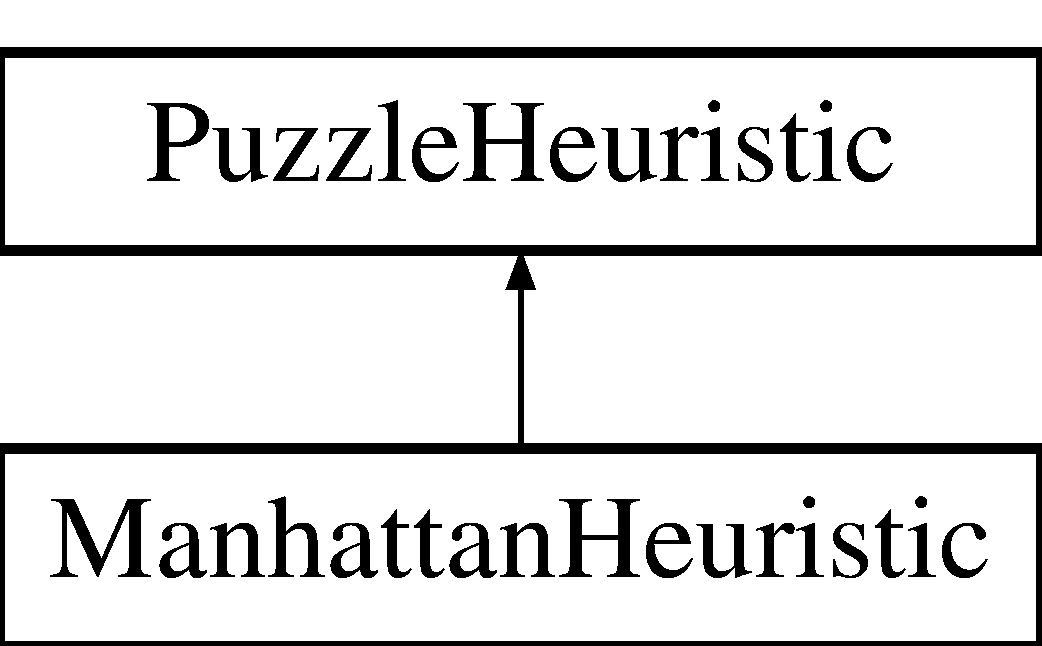
\includegraphics[height=2.000000cm]{classManhattanHeuristic}
\end{center}
\end{figure}
\subsection*{\-Public \-Member \-Functions}
\begin{DoxyCompactItemize}
\item 
int \hyperlink{classManhattanHeuristic_a061af5e85bffa6a6f7cebbce17f5e7e5}{compute} (int $\ast$tiles, int size)
\end{DoxyCompactItemize}


\subsection{\-Member \-Function \-Documentation}
\hypertarget{classManhattanHeuristic_a061af5e85bffa6a6f7cebbce17f5e7e5}{\index{\-Manhattan\-Heuristic@{\-Manhattan\-Heuristic}!compute@{compute}}
\index{compute@{compute}!ManhattanHeuristic@{\-Manhattan\-Heuristic}}
\subsubsection[{compute}]{\setlength{\rightskip}{0pt plus 5cm}int {\bf \-Manhattan\-Heuristic\-::compute} (
\begin{DoxyParamCaption}
\item[{int $\ast$}]{tiles, }
\item[{int}]{size}
\end{DoxyParamCaption}
)\hspace{0.3cm}{\ttfamily  \mbox{[}virtual\mbox{]}}}}\label{classManhattanHeuristic_a061af5e85bffa6a6f7cebbce17f5e7e5}
\-Compute h score by using manhattan heuristic 
\begin{DoxyParams}{\-Parameters}
{\em tiles} & \-Tiles of right hand side board class \\
\hline
{\em size} & \-Size of right hand side board class \\
\hline
\end{DoxyParams}
\begin{DoxyReturn}{\-Returns}
\-Computed h score 
\end{DoxyReturn}


\-Implements \hyperlink{classPuzzleHeuristic_ada41c4cd5106f0d1756c4d5886731c6c}{\-Puzzle\-Heuristic}.



\-The documentation for this class was generated from the following files\-:\begin{DoxyCompactItemize}
\item 
puzzle\-\_\-heur.\-h\item 
puzzle\-\_\-heur.\-cpp\end{DoxyCompactItemize}

\hypertarget{classMyList}{\section{\-My\-List$<$ \-T $>$ \-Class \-Template \-Reference}
\label{classMyList}\index{\-My\-List$<$ T $>$@{\-My\-List$<$ T $>$}}
}
\subsection*{\-Public \-Member \-Functions}
\begin{DoxyCompactItemize}
\item 
\hyperlink{classMyList_aaa11039853c7adb2fbcb770eab8b7305}{\-My\-List} ()
\item 
\hyperlink{classMyList_a43e0aa06b56b08ab65d9f8b7086aeb92}{\-My\-List} (int capacity)
\item 
\hyperlink{classMyList_aa622b9fb3e108b8b8c298ef1996dd256}{$\sim$\-My\-List} ()
\item 
void \hyperlink{classMyList_a55eebaa813ab6e221b5a7c25c790c9d2}{push\-\_\-back} (\-T newval)
\item 
\-T \& \hyperlink{classMyList_aede5c62a87c09cd4c7a36ad34d55fb9d}{at} (int loc)
\item 
int \hyperlink{classMyList_a290dc305556aadc0d4c68b456987a7d0}{size} () const 
\item 
bool \hyperlink{classMyList_a7f8a0f53d5153886cb5d6dcca9a07ff3}{remove} (\-T val)
\item 
\-T \hyperlink{classMyList_aca4ff0b35241e2a7e3953b123621e2fb}{pop} (int loc)
\item 
\-T \& \hyperlink{classMyList_ac042422a2d7dcc3fb90eda17f5e2970a}{operator\mbox{[}$\,$\mbox{]}} (int loc)
\item 
\-T \hyperlink{classMyList_a4f422fc82b3b0a94788d3792d4dba57c}{max} () const 
\item 
\-T \hyperlink{classMyList_a8718b2b826ee315d3f730cf52193b11e}{min} () const 
\item 
void \hyperlink{classMyList_a6e671ba282372c9280fbdb1b0852cd80}{pop\-\_\-back} ()
\end{DoxyCompactItemize}
\subsubsection*{template$<$typename \-T$>$ class My\-List$<$ T $>$}



\subsection{\-Constructor \& \-Destructor \-Documentation}
\hypertarget{classMyList_aaa11039853c7adb2fbcb770eab8b7305}{\index{\-My\-List@{\-My\-List}!\-My\-List@{\-My\-List}}
\index{\-My\-List@{\-My\-List}!MyList@{\-My\-List}}
\subsubsection[{\-My\-List}]{\setlength{\rightskip}{0pt plus 5cm}template$<$typename T $>$ {\bf \-My\-List}$<$ \-T $>$\-::{\bf \-My\-List} (
\begin{DoxyParamCaption}
{}
\end{DoxyParamCaption}
)}}\label{classMyList_aaa11039853c7adb2fbcb770eab8b7305}
\-Default constructor \-Initialize capacity, size, and date \hypertarget{classMyList_a43e0aa06b56b08ab65d9f8b7086aeb92}{\index{\-My\-List@{\-My\-List}!\-My\-List@{\-My\-List}}
\index{\-My\-List@{\-My\-List}!MyList@{\-My\-List}}
\subsubsection[{\-My\-List}]{\setlength{\rightskip}{0pt plus 5cm}template$<$typename T $>$ {\bf \-My\-List}$<$ \-T $>$\-::{\bf \-My\-List} (
\begin{DoxyParamCaption}
\item[{int}]{capacity}
\end{DoxyParamCaption}
)}}\label{classMyList_a43e0aa06b56b08ab65d9f8b7086aeb92}
\-Constructor \-Initialize capacity, size, and date when capacity is given \hypertarget{classMyList_aa622b9fb3e108b8b8c298ef1996dd256}{\index{\-My\-List@{\-My\-List}!$\sim$\-My\-List@{$\sim$\-My\-List}}
\index{$\sim$\-My\-List@{$\sim$\-My\-List}!MyList@{\-My\-List}}
\subsubsection[{$\sim$\-My\-List}]{\setlength{\rightskip}{0pt plus 5cm}template$<$typename T $>$ {\bf \-My\-List}$<$ \-T $>$\-::$\sim${\bf \-My\-List} (
\begin{DoxyParamCaption}
{}
\end{DoxyParamCaption}
)}}\label{classMyList_aa622b9fb3e108b8b8c298ef1996dd256}
\-Destructor 

\subsection{\-Member \-Function \-Documentation}
\hypertarget{classMyList_aede5c62a87c09cd4c7a36ad34d55fb9d}{\index{\-My\-List@{\-My\-List}!at@{at}}
\index{at@{at}!MyList@{\-My\-List}}
\subsubsection[{at}]{\setlength{\rightskip}{0pt plus 5cm}template$<$typename T $>$ \-T \& {\bf \-My\-List}$<$ \-T $>$\-::{\bf at} (
\begin{DoxyParamCaption}
\item[{int}]{loc}
\end{DoxyParamCaption}
)}}\label{classMyList_aede5c62a87c09cd4c7a36ad34d55fb9d}
\-Return the value at particular location 
\begin{DoxyParams}{\-Parameters}
{\em loc} & \-Loaction number \\
\hline
\end{DoxyParams}
\begin{DoxyReturn}{\-Returns}
\-Value at the location 
\end{DoxyReturn}
\hypertarget{classMyList_a4f422fc82b3b0a94788d3792d4dba57c}{\index{\-My\-List@{\-My\-List}!max@{max}}
\index{max@{max}!MyList@{\-My\-List}}
\subsubsection[{max}]{\setlength{\rightskip}{0pt plus 5cm}template$<$typename T $>$ \-T {\bf \-My\-List}$<$ \-T $>$\-::{\bf max} (
\begin{DoxyParamCaption}
{}
\end{DoxyParamCaption}
) const}}\label{classMyList_a4f422fc82b3b0a94788d3792d4dba57c}
\-Return the biggest value in the list \begin{DoxyReturn}{\-Returns}
\-Maximum value 
\end{DoxyReturn}
\hypertarget{classMyList_a8718b2b826ee315d3f730cf52193b11e}{\index{\-My\-List@{\-My\-List}!min@{min}}
\index{min@{min}!MyList@{\-My\-List}}
\subsubsection[{min}]{\setlength{\rightskip}{0pt plus 5cm}template$<$typename T $>$ \-T {\bf \-My\-List}$<$ \-T $>$\-::{\bf min} (
\begin{DoxyParamCaption}
{}
\end{DoxyParamCaption}
) const}}\label{classMyList_a8718b2b826ee315d3f730cf52193b11e}
\-Return the smallest value in the list \begin{DoxyReturn}{\-Returns}
\-Smallest value 
\end{DoxyReturn}
\hypertarget{classMyList_ac042422a2d7dcc3fb90eda17f5e2970a}{\index{\-My\-List@{\-My\-List}!operator\mbox{[}$\,$\mbox{]}@{operator[]}}
\index{operator\mbox{[}$\,$\mbox{]}@{operator[]}!MyList@{\-My\-List}}
\subsubsection[{operator[]}]{\setlength{\rightskip}{0pt plus 5cm}template$<$typename T $>$ \-T \& {\bf \-My\-List}$<$ \-T $>$\-::operator\mbox{[}$\,$\mbox{]} (
\begin{DoxyParamCaption}
\item[{int}]{loc}
\end{DoxyParamCaption}
)}}\label{classMyList_ac042422a2d7dcc3fb90eda17f5e2970a}
\-Operater for \mbox{[}\mbox{]} \hypertarget{classMyList_aca4ff0b35241e2a7e3953b123621e2fb}{\index{\-My\-List@{\-My\-List}!pop@{pop}}
\index{pop@{pop}!MyList@{\-My\-List}}
\subsubsection[{pop}]{\setlength{\rightskip}{0pt plus 5cm}template$<$typename T $>$ \-T {\bf \-My\-List}$<$ \-T $>$\-::{\bf pop} (
\begin{DoxyParamCaption}
\item[{int}]{loc}
\end{DoxyParamCaption}
)}}\label{classMyList_aca4ff0b35241e2a7e3953b123621e2fb}
\-Return the value at particular location and remove it 
\begin{DoxyParams}{\-Parameters}
{\em loc} & \-Location that will be returned and deleted \\
\hline
\end{DoxyParams}
\begin{DoxyReturn}{\-Returns}
\-Value at entered location 
\end{DoxyReturn}
\hypertarget{classMyList_a6e671ba282372c9280fbdb1b0852cd80}{\index{\-My\-List@{\-My\-List}!pop\-\_\-back@{pop\-\_\-back}}
\index{pop\-\_\-back@{pop\-\_\-back}!MyList@{\-My\-List}}
\subsubsection[{pop\-\_\-back}]{\setlength{\rightskip}{0pt plus 5cm}template$<$typename T $>$ void {\bf \-My\-List}$<$ \-T $>$\-::{\bf pop\-\_\-back} (
\begin{DoxyParamCaption}
{}
\end{DoxyParamCaption}
)}}\label{classMyList_a6e671ba282372c9280fbdb1b0852cd80}
\-Delete the most back of list \hypertarget{classMyList_a55eebaa813ab6e221b5a7c25c790c9d2}{\index{\-My\-List@{\-My\-List}!push\-\_\-back@{push\-\_\-back}}
\index{push\-\_\-back@{push\-\_\-back}!MyList@{\-My\-List}}
\subsubsection[{push\-\_\-back}]{\setlength{\rightskip}{0pt plus 5cm}template$<$typename \-T$>$ void {\bf \-My\-List}$<$ \-T $>$\-::{\bf push\-\_\-back} (
\begin{DoxyParamCaption}
\item[{\-T}]{newval}
\end{DoxyParamCaption}
)}}\label{classMyList_a55eebaa813ab6e221b5a7c25c790c9d2}
\-Push back new value to the list 
\begin{DoxyParams}{\-Parameters}
{\em newval} & \-New value that will be inserted at the back of list \\
\hline
\end{DoxyParams}
\begin{DoxyReturn}{\-Returns}
\-Nothing 
\end{DoxyReturn}
\hypertarget{classMyList_a7f8a0f53d5153886cb5d6dcca9a07ff3}{\index{\-My\-List@{\-My\-List}!remove@{remove}}
\index{remove@{remove}!MyList@{\-My\-List}}
\subsubsection[{remove}]{\setlength{\rightskip}{0pt plus 5cm}template$<$typename \-T$>$ bool {\bf \-My\-List}$<$ \-T $>$\-::{\bf remove} (
\begin{DoxyParamCaption}
\item[{\-T}]{val}
\end{DoxyParamCaption}
)}}\label{classMyList_a7f8a0f53d5153886cb5d6dcca9a07ff3}
\-Remove particular value if that value is in the list. \par
 \-Return true if that value exist, and false if does not exist. 
\begin{DoxyParams}{\-Parameters}
{\em val} & \-Value that will be deleted if the same value is in the list \\
\hline
\end{DoxyParams}
\begin{DoxyReturn}{\-Returns}
\-True or \-False according to the result 
\end{DoxyReturn}
\hypertarget{classMyList_a290dc305556aadc0d4c68b456987a7d0}{\index{\-My\-List@{\-My\-List}!size@{size}}
\index{size@{size}!MyList@{\-My\-List}}
\subsubsection[{size}]{\setlength{\rightskip}{0pt plus 5cm}template$<$typename T $>$ int {\bf \-My\-List}$<$ \-T $>$\-::{\bf size} (
\begin{DoxyParamCaption}
{}
\end{DoxyParamCaption}
) const}}\label{classMyList_a290dc305556aadc0d4c68b456987a7d0}
\-Return the size of mylist \begin{DoxyReturn}{\-Returns}
\-Size of mylist 
\end{DoxyReturn}


\-The documentation for this class was generated from the following file\-:\begin{DoxyCompactItemize}
\item 
mylist.\-h\end{DoxyCompactItemize}

\hypertarget{classOutOfPlaceHeuristic}{\section{\-Out\-Of\-Place\-Heuristic \-Class \-Reference}
\label{classOutOfPlaceHeuristic}\index{\-Out\-Of\-Place\-Heuristic@{\-Out\-Of\-Place\-Heuristic}}
}
\-Inheritance diagram for \-Out\-Of\-Place\-Heuristic\-:\begin{figure}[H]
\begin{center}
\leavevmode
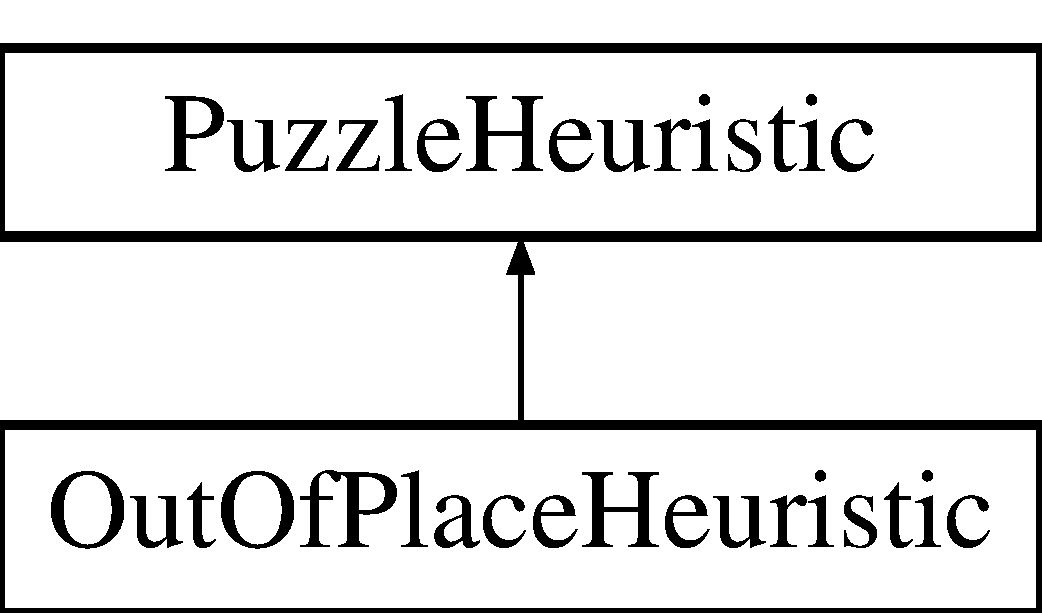
\includegraphics[height=2.000000cm]{classOutOfPlaceHeuristic}
\end{center}
\end{figure}
\subsection*{\-Public \-Member \-Functions}
\begin{DoxyCompactItemize}
\item 
int \hyperlink{classOutOfPlaceHeuristic_acc042925c642807a995a18ee3393098d}{compute} (int $\ast$tiles, int size)
\end{DoxyCompactItemize}


\subsection{\-Member \-Function \-Documentation}
\hypertarget{classOutOfPlaceHeuristic_acc042925c642807a995a18ee3393098d}{\index{\-Out\-Of\-Place\-Heuristic@{\-Out\-Of\-Place\-Heuristic}!compute@{compute}}
\index{compute@{compute}!OutOfPlaceHeuristic@{\-Out\-Of\-Place\-Heuristic}}
\subsubsection[{compute}]{\setlength{\rightskip}{0pt plus 5cm}int {\bf \-Out\-Of\-Place\-Heuristic\-::compute} (
\begin{DoxyParamCaption}
\item[{int $\ast$}]{tiles, }
\item[{int}]{size}
\end{DoxyParamCaption}
)\hspace{0.3cm}{\ttfamily  \mbox{[}virtual\mbox{]}}}}\label{classOutOfPlaceHeuristic_acc042925c642807a995a18ee3393098d}
\-Compute h score by using out-\/of-\/place heuristic 
\begin{DoxyParams}{\-Parameters}
{\em tiles} & \-Tiles of right hand side board class \\
\hline
{\em size} & \-Size of right hand side board class \\
\hline
\end{DoxyParams}
\begin{DoxyReturn}{\-Returns}
\-Computed h score 
\end{DoxyReturn}


\-Implements \hyperlink{classPuzzleHeuristic_ada41c4cd5106f0d1756c4d5886731c6c}{\-Puzzle\-Heuristic}.



\-The documentation for this class was generated from the following files\-:\begin{DoxyCompactItemize}
\item 
puzzle\-\_\-heur.\-h\item 
puzzle\-\_\-heur.\-cpp\end{DoxyCompactItemize}

\hypertarget{classPMMinList}{\section{\-P\-M\-Min\-List \-Class \-Reference}
\label{classPMMinList}\index{\-P\-M\-Min\-List@{\-P\-M\-Min\-List}}
}


{\ttfamily \#include $<$pmminlist.\-h$>$}

\subsection*{\-Public \-Member \-Functions}
\begin{DoxyCompactItemize}
\item 
\hyperlink{classPMMinList_a1fa1ed01cc65ea09cdd9bd10198fabee}{\-P\-M\-Min\-List} ()
\item 
\hyperlink{classPMMinList_a886c0f8fe079a8353c23da4ff163beae}{$\sim$\-P\-M\-Min\-List} ()
\item 
int \hyperlink{classPMMinList_a692220d438ffab3cf6729de3dc38c1fb}{size} () const 
\item 
bool \hyperlink{classPMMinList_a1c148a978af1a6ea964ee7141a80855e}{empty} () const 
\item 
void \hyperlink{classPMMinList_aafa81672d5dd017bf5e6f76b65022d21}{push} (\hyperlink{classPuzzleMove}{\-Puzzle\-Move} $\ast$pm)
\item 
void \hyperlink{classPMMinList_a77fa8f64f75cc6c1469688928d372089}{pop} ()
\item 
\hyperlink{classPuzzleMove}{\-Puzzle\-Move} $\ast$ \hyperlink{classPMMinList_a6a04fe787c09097ecd3a76428a3524ba}{top} ()
\end{DoxyCompactItemize}


\subsection{\-Detailed \-Description}
\hyperlink{classPMMinList}{\-P\-M\-Min\-List} implements a sorted list of \-Puzzle\-Moves based on their f-\/score (from smallest to largest) 

\subsection{\-Constructor \& \-Destructor \-Documentation}
\hypertarget{classPMMinList_a1fa1ed01cc65ea09cdd9bd10198fabee}{\index{\-P\-M\-Min\-List@{\-P\-M\-Min\-List}!\-P\-M\-Min\-List@{\-P\-M\-Min\-List}}
\index{\-P\-M\-Min\-List@{\-P\-M\-Min\-List}!PMMinList@{\-P\-M\-Min\-List}}
\subsubsection[{\-P\-M\-Min\-List}]{\setlength{\rightskip}{0pt plus 5cm}{\bf \-P\-M\-Min\-List\-::\-P\-M\-Min\-List} (
\begin{DoxyParamCaption}
{}
\end{DoxyParamCaption}
)}}\label{classPMMinList_a1fa1ed01cc65ea09cdd9bd10198fabee}
\-Default \-Constructor \hypertarget{classPMMinList_a886c0f8fe079a8353c23da4ff163beae}{\index{\-P\-M\-Min\-List@{\-P\-M\-Min\-List}!$\sim$\-P\-M\-Min\-List@{$\sim$\-P\-M\-Min\-List}}
\index{$\sim$\-P\-M\-Min\-List@{$\sim$\-P\-M\-Min\-List}!PMMinList@{\-P\-M\-Min\-List}}
\subsubsection[{$\sim$\-P\-M\-Min\-List}]{\setlength{\rightskip}{0pt plus 5cm}{\bf \-P\-M\-Min\-List\-::$\sim$\-P\-M\-Min\-List} (
\begin{DoxyParamCaption}
{}
\end{DoxyParamCaption}
)}}\label{classPMMinList_a886c0f8fe079a8353c23da4ff163beae}
\-Destructor 

\subsection{\-Member \-Function \-Documentation}
\hypertarget{classPMMinList_a1c148a978af1a6ea964ee7141a80855e}{\index{\-P\-M\-Min\-List@{\-P\-M\-Min\-List}!empty@{empty}}
\index{empty@{empty}!PMMinList@{\-P\-M\-Min\-List}}
\subsubsection[{empty}]{\setlength{\rightskip}{0pt plus 5cm}bool {\bf \-P\-M\-Min\-List\-::empty} (
\begin{DoxyParamCaption}
{}
\end{DoxyParamCaption}
) const\hspace{0.3cm}{\ttfamily  \mbox{[}inline\mbox{]}}}}\label{classPMMinList_a1c148a978af1a6ea964ee7141a80855e}
\-Returns true if the list is empty \hypertarget{classPMMinList_a77fa8f64f75cc6c1469688928d372089}{\index{\-P\-M\-Min\-List@{\-P\-M\-Min\-List}!pop@{pop}}
\index{pop@{pop}!PMMinList@{\-P\-M\-Min\-List}}
\subsubsection[{pop}]{\setlength{\rightskip}{0pt plus 5cm}void {\bf \-P\-M\-Min\-List\-::pop} (
\begin{DoxyParamCaption}
{}
\end{DoxyParamCaption}
)}}\label{classPMMinList_a77fa8f64f75cc6c1469688928d372089}
\-Removes the minimum scored (front) puzzle move

\-Removes the top (minimum) item \begin{DoxyReturn}{\-Returns}
nothing 
\end{DoxyReturn}
\hypertarget{classPMMinList_aafa81672d5dd017bf5e6f76b65022d21}{\index{\-P\-M\-Min\-List@{\-P\-M\-Min\-List}!push@{push}}
\index{push@{push}!PMMinList@{\-P\-M\-Min\-List}}
\subsubsection[{push}]{\setlength{\rightskip}{0pt plus 5cm}void {\bf \-P\-M\-Min\-List\-::push} (
\begin{DoxyParamCaption}
\item[{{\bf \-Puzzle\-Move} $\ast$}]{pm}
\end{DoxyParamCaption}
)}}\label{classPMMinList_aafa81672d5dd017bf5e6f76b65022d21}
\-Adds a puzzle move to the sorted list

\-Adds the value val to the internal list in sorted order from smallest to largest (if 
\begin{DoxyParams}{\-Parameters}
{\em val} & \-Value to add to the sorted \hyperlink{classPuzzleMove}{\-Puzzle\-Move} list \\
\hline
\end{DoxyParams}
\begin{DoxyReturn}{\-Returns}
nothing 
\end{DoxyReturn}
\hypertarget{classPMMinList_a692220d438ffab3cf6729de3dc38c1fb}{\index{\-P\-M\-Min\-List@{\-P\-M\-Min\-List}!size@{size}}
\index{size@{size}!PMMinList@{\-P\-M\-Min\-List}}
\subsubsection[{size}]{\setlength{\rightskip}{0pt plus 5cm}int {\bf \-P\-M\-Min\-List\-::size} (
\begin{DoxyParamCaption}
{}
\end{DoxyParamCaption}
) const\hspace{0.3cm}{\ttfamily  \mbox{[}inline\mbox{]}}}}\label{classPMMinList_a692220d438ffab3cf6729de3dc38c1fb}
\-Returns the size of items in the list \hypertarget{classPMMinList_a6a04fe787c09097ecd3a76428a3524ba}{\index{\-P\-M\-Min\-List@{\-P\-M\-Min\-List}!top@{top}}
\index{top@{top}!PMMinList@{\-P\-M\-Min\-List}}
\subsubsection[{top}]{\setlength{\rightskip}{0pt plus 5cm}{\bf \-Puzzle\-Move} $\ast$ {\bf \-P\-M\-Min\-List\-::top} (
\begin{DoxyParamCaption}
{}
\end{DoxyParamCaption}
)}}\label{classPMMinList_a6a04fe787c09097ecd3a76428a3524ba}
\-Returns the \hyperlink{classPuzzleMove}{\-Puzzle\-Move} with the lowest score

\-Returns the top (minimum) item \begin{DoxyReturn}{\-Returns}
pointer to the minimum-\/scored \hyperlink{classPuzzleMove}{\-Puzzle\-Move} 
\end{DoxyReturn}


\-The documentation for this class was generated from the following files\-:\begin{DoxyCompactItemize}
\item 
pmminlist.\-h\item 
pmminlist.\-cpp\end{DoxyCompactItemize}

\hypertarget{classPuzzleHeuristic}{\section{\-Puzzle\-Heuristic \-Class \-Reference}
\label{classPuzzleHeuristic}\index{\-Puzzle\-Heuristic@{\-Puzzle\-Heuristic}}
}
\-Inheritance diagram for \-Puzzle\-Heuristic\-:\begin{figure}[H]
\begin{center}
\leavevmode
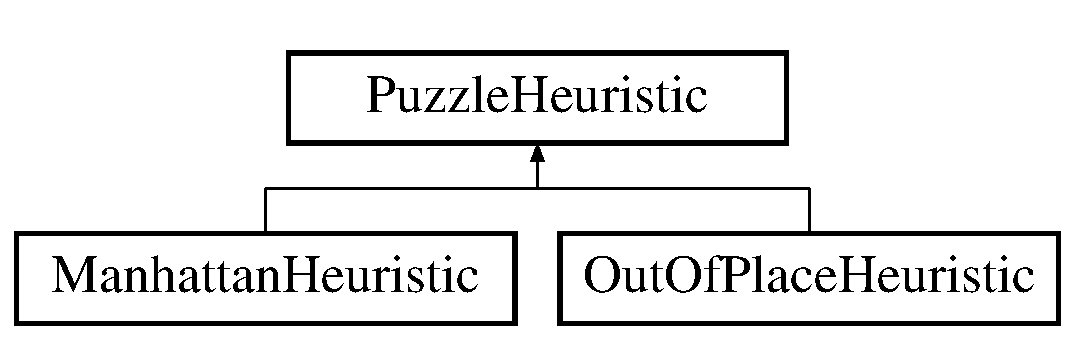
\includegraphics[height=2.000000cm]{classPuzzleHeuristic}
\end{center}
\end{figure}
\subsection*{\-Public \-Member \-Functions}
\begin{DoxyCompactItemize}
\item 
virtual int \hyperlink{classPuzzleHeuristic_ada41c4cd5106f0d1756c4d5886731c6c}{compute} (int $\ast$tiles, int size)=0
\end{DoxyCompactItemize}


\subsection{\-Member \-Function \-Documentation}
\hypertarget{classPuzzleHeuristic_ada41c4cd5106f0d1756c4d5886731c6c}{\index{\-Puzzle\-Heuristic@{\-Puzzle\-Heuristic}!compute@{compute}}
\index{compute@{compute}!PuzzleHeuristic@{\-Puzzle\-Heuristic}}
\subsubsection[{compute}]{\setlength{\rightskip}{0pt plus 5cm}virtual int {\bf \-Puzzle\-Heuristic\-::compute} (
\begin{DoxyParamCaption}
\item[{int $\ast$}]{tiles, }
\item[{int}]{size}
\end{DoxyParamCaption}
)\hspace{0.3cm}{\ttfamily  \mbox{[}pure virtual\mbox{]}}}}\label{classPuzzleHeuristic_ada41c4cd5106f0d1756c4d5886731c6c}
\-Compute h score either by manhattan heuristic or out-\/of-\/place heuristic \par
 \-Virtual function for the compute 
\begin{DoxyParams}{\-Parameters}
{\em tiles} & \-Tiles of right hand side board class \\
\hline
{\em size} & \-Size of right hand side board class \\
\hline
\end{DoxyParams}
\begin{DoxyReturn}{\-Returns}
\-Computed h score 
\end{DoxyReturn}


\-Implemented in \hyperlink{classOutOfPlaceHeuristic_acc042925c642807a995a18ee3393098d}{\-Out\-Of\-Place\-Heuristic}, and \hyperlink{classManhattanHeuristic_a061af5e85bffa6a6f7cebbce17f5e7e5}{\-Manhattan\-Heuristic}.



\-The documentation for this class was generated from the following file\-:\begin{DoxyCompactItemize}
\item 
puzzle\-\_\-heur.\-h\end{DoxyCompactItemize}

\hypertarget{classPuzzleMove}{\section{\-Puzzle\-Move \-Class \-Reference}
\label{classPuzzleMove}\index{\-Puzzle\-Move@{\-Puzzle\-Move}}
}
\subsection*{\-Public \-Member \-Functions}
\begin{DoxyCompactItemize}
\item 
\hyperlink{classPuzzleMove_aab82684bd0bec53818b36ff1d38cd918}{\-Puzzle\-Move} (\hyperlink{classBoard}{\-Board} \&b)
\item 
\hyperlink{classPuzzleMove_a648f58dc747438872988d888b1b91c35}{\-Puzzle\-Move} (int tile, \hyperlink{classBoard}{\-Board} $\ast$b, \hyperlink{classPuzzleMove}{\-Puzzle\-Move} $\ast$parent)
\item 
\hypertarget{classPuzzleMove_a3b76cc463e70c40feed64915363c3dd9}{bool {\bfseries operator$<$} (const \hyperlink{classPuzzleMove}{\-Puzzle\-Move} \&p) const }\label{classPuzzleMove_a3b76cc463e70c40feed64915363c3dd9}

\item 
\hypertarget{classPuzzleMove_acdbbc19713741a1adf74e6886b52a6d7}{bool {\bfseries operator$>$} (const \hyperlink{classPuzzleMove}{\-Puzzle\-Move} \&p) const }\label{classPuzzleMove_acdbbc19713741a1adf74e6886b52a6d7}

\item 
\hypertarget{classPuzzleMove_abd3fe605a9546d8ff7cc4609cef69761}{bool {\bfseries operator==} (const \hyperlink{classPuzzleMove}{\-Puzzle\-Move} \&p) const }\label{classPuzzleMove_abd3fe605a9546d8ff7cc4609cef69761}

\end{DoxyCompactItemize}
\subsection*{\-Public \-Attributes}
\begin{DoxyCompactItemize}
\item 
\hypertarget{classPuzzleMove_aa2fffc45e00d35346c0f88cab11b8e5a}{int {\bfseries tile\-Move\-\_\-}}\label{classPuzzleMove_aa2fffc45e00d35346c0f88cab11b8e5a}

\item 
\hypertarget{classPuzzleMove_a31158ed0a7fa5c8d814cdedb0369e358}{\hyperlink{classBoard}{\-Board} $\ast$ {\bfseries b\-\_\-}}\label{classPuzzleMove_a31158ed0a7fa5c8d814cdedb0369e358}

\item 
\hypertarget{classPuzzleMove_a5447ee712ef759570d47dd585bfd4ee2}{int {\bfseries g\-\_\-}}\label{classPuzzleMove_a5447ee712ef759570d47dd585bfd4ee2}

\item 
\hypertarget{classPuzzleMove_a15335bf6718edc6ccf4577d0352d8deb}{int {\bfseries h\-\_\-}}\label{classPuzzleMove_a15335bf6718edc6ccf4577d0352d8deb}

\item 
\hypertarget{classPuzzleMove_a717d4e75b18720e43cf207cfca84b834}{int {\bfseries f\-\_\-}}\label{classPuzzleMove_a717d4e75b18720e43cf207cfca84b834}

\item 
\hypertarget{classPuzzleMove_a316ee56f76f0f21b61a9f4d027215f1e}{\hyperlink{classPuzzleMove}{\-Puzzle\-Move} $\ast$ {\bfseries prev\-\_\-}}\label{classPuzzleMove_a316ee56f76f0f21b61a9f4d027215f1e}

\end{DoxyCompactItemize}


\subsection{\-Constructor \& \-Destructor \-Documentation}
\hypertarget{classPuzzleMove_aab82684bd0bec53818b36ff1d38cd918}{\index{\-Puzzle\-Move@{\-Puzzle\-Move}!\-Puzzle\-Move@{\-Puzzle\-Move}}
\index{\-Puzzle\-Move@{\-Puzzle\-Move}!PuzzleMove@{\-Puzzle\-Move}}
\subsubsection[{\-Puzzle\-Move}]{\setlength{\rightskip}{0pt plus 5cm}{\bf \-Puzzle\-Move\-::\-Puzzle\-Move} (
\begin{DoxyParamCaption}
\item[{{\bf \-Board} \&}]{b}
\end{DoxyParamCaption}
)}}\label{classPuzzleMove_aab82684bd0bec53818b36ff1d38cd918}
\-Constructor for starting \hyperlink{classBoard}{\-Board} of an \-A$\ast$ search @ param b \hypertarget{classPuzzleMove_a648f58dc747438872988d888b1b91c35}{\index{\-Puzzle\-Move@{\-Puzzle\-Move}!\-Puzzle\-Move@{\-Puzzle\-Move}}
\index{\-Puzzle\-Move@{\-Puzzle\-Move}!PuzzleMove@{\-Puzzle\-Move}}
\subsubsection[{\-Puzzle\-Move}]{\setlength{\rightskip}{0pt plus 5cm}{\bf \-Puzzle\-Move\-::\-Puzzle\-Move} (
\begin{DoxyParamCaption}
\item[{int}]{tile, }
\item[{{\bf \-Board} $\ast$}]{b, }
\item[{{\bf \-Puzzle\-Move} $\ast$}]{parent}
\end{DoxyParamCaption}
)}}\label{classPuzzleMove_a648f58dc747438872988d888b1b91c35}
\-Constructor for subsequent search boards (i.\-e. those returned by \hyperlink{classBoard_a69149b8091bfaf02a394bedb9ff5f57f}{\-Board\-::potential\-Moves()} ) 

\-The documentation for this class was generated from the following files\-:\begin{DoxyCompactItemize}
\item 
puzzle\-\_\-move.\-h\item 
puzzle\-\_\-move.\-cpp\end{DoxyCompactItemize}

\hypertarget{structPuzzleMoveGreater}{\section{\-Puzzle\-Move\-Greater \-Struct \-Reference}
\label{structPuzzleMoveGreater}\index{\-Puzzle\-Move\-Greater@{\-Puzzle\-Move\-Greater}}
}
\subsection*{\-Public \-Member \-Functions}
\begin{DoxyCompactItemize}
\item 
\hypertarget{structPuzzleMoveGreater_a43793ecee311b7522d2f7507cca025ac}{bool {\bfseries operator()} (const \hyperlink{classPuzzleMove}{\-Puzzle\-Move} $\ast$m1, const \hyperlink{classPuzzleMove}{\-Puzzle\-Move} $\ast$m2) const }\label{structPuzzleMoveGreater_a43793ecee311b7522d2f7507cca025ac}

\end{DoxyCompactItemize}


\-The documentation for this struct was generated from the following file\-:\begin{DoxyCompactItemize}
\item 
puzzle\-\_\-move.\-h\end{DoxyCompactItemize}

\hypertarget{classPuzzleSolver}{\section{\-Puzzle\-Solver \-Class \-Reference}
\label{classPuzzleSolver}\index{\-Puzzle\-Solver@{\-Puzzle\-Solver}}
}
\subsection*{\-Public \-Types}
\begin{DoxyCompactItemize}
\item 
typedef std\-::set$<$ \hyperlink{classBoard}{\-Board} \*
$\ast$, \hyperlink{structBoardLessThan}{\-Board\-Less\-Than} $>$ \hyperlink{classPuzzleSolver_a868921fe5292af6190a7bc068e32a2c7}{\-Board\-Set}
\end{DoxyCompactItemize}
\subsection*{\-Public \-Member \-Functions}
\begin{DoxyCompactItemize}
\item 
\hyperlink{classPuzzleSolver_a70e86dbac90a3c6567598cb02fc523f2}{\-Puzzle\-Solver} (const \hyperlink{classBoard}{\-Board} \&b)
\item 
\hyperlink{classPuzzleSolver_adcc789feca768f7d468f6ca8806f75a3}{$\sim$\-Puzzle\-Solver} ()
\item 
int \hyperlink{classPuzzleSolver_a99e867d21204e8958f0bdfbcbbd01c5f}{run} (\hyperlink{classPuzzleHeuristic}{\-Puzzle\-Heuristic} $\ast$ph)
\item 
deque$<$ int $>$ \hyperlink{classPuzzleSolver_a92a5a1bba3ca6bc46d44d26b9bcf41cc}{get\-\_\-solution} ()
\item 
int \hyperlink{classPuzzleSolver_a2aa96aa4631d4a4b295fddf49e5dd9f7}{get\-Num\-Expansions} ()
\end{DoxyCompactItemize}


\subsection{\-Member \-Typedef \-Documentation}
\hypertarget{classPuzzleSolver_a868921fe5292af6190a7bc068e32a2c7}{\index{\-Puzzle\-Solver@{\-Puzzle\-Solver}!\-Board\-Set@{\-Board\-Set}}
\index{\-Board\-Set@{\-Board\-Set}!PuzzleSolver@{\-Puzzle\-Solver}}
\subsubsection[{\-Board\-Set}]{\setlength{\rightskip}{0pt plus 5cm}typedef std\-::set$<${\bf \-Board} $\ast$, {\bf \-Board\-Less\-Than}$>$ {\bf \-Puzzle\-Solver\-::\-Board\-Set}}}\label{classPuzzleSolver_a868921fe5292af6190a7bc068e32a2c7}
\-Typedef for the closed-\/list set. 

\subsection{\-Constructor \& \-Destructor \-Documentation}
\hypertarget{classPuzzleSolver_a70e86dbac90a3c6567598cb02fc523f2}{\index{\-Puzzle\-Solver@{\-Puzzle\-Solver}!\-Puzzle\-Solver@{\-Puzzle\-Solver}}
\index{\-Puzzle\-Solver@{\-Puzzle\-Solver}!PuzzleSolver@{\-Puzzle\-Solver}}
\subsubsection[{\-Puzzle\-Solver}]{\setlength{\rightskip}{0pt plus 5cm}{\bf \-Puzzle\-Solver\-::\-Puzzle\-Solver} (
\begin{DoxyParamCaption}
\item[{const {\bf \-Board} \&}]{b}
\end{DoxyParamCaption}
)}}\label{classPuzzleSolver_a70e86dbac90a3c6567598cb02fc523f2}
\-Constructor (makes a copy of the \hyperlink{classBoard}{\-Board} and stores it in \-\_\-b \hypertarget{classPuzzleSolver_adcc789feca768f7d468f6ca8806f75a3}{\index{\-Puzzle\-Solver@{\-Puzzle\-Solver}!$\sim$\-Puzzle\-Solver@{$\sim$\-Puzzle\-Solver}}
\index{$\sim$\-Puzzle\-Solver@{$\sim$\-Puzzle\-Solver}!PuzzleSolver@{\-Puzzle\-Solver}}
\subsubsection[{$\sim$\-Puzzle\-Solver}]{\setlength{\rightskip}{0pt plus 5cm}{\bf \-Puzzle\-Solver\-::$\sim$\-Puzzle\-Solver} (
\begin{DoxyParamCaption}
{}
\end{DoxyParamCaption}
)}}\label{classPuzzleSolver_adcc789feca768f7d468f6ca8806f75a3}
\-Destructor 

\subsection{\-Member \-Function \-Documentation}
\hypertarget{classPuzzleSolver_a92a5a1bba3ca6bc46d44d26b9bcf41cc}{\index{\-Puzzle\-Solver@{\-Puzzle\-Solver}!get\-\_\-solution@{get\-\_\-solution}}
\index{get\-\_\-solution@{get\-\_\-solution}!PuzzleSolver@{\-Puzzle\-Solver}}
\subsubsection[{get\-\_\-solution}]{\setlength{\rightskip}{0pt plus 5cm}deque$<$ int $>$ {\bf \-Puzzle\-Solver\-::get\-\_\-solution} (
\begin{DoxyParamCaption}
{}
\end{DoxyParamCaption}
)}}\label{classPuzzleSolver_a92a5a1bba3ca6bc46d44d26b9bcf41cc}
\-Return the list of solution tile number \hypertarget{classPuzzleSolver_a2aa96aa4631d4a4b295fddf49e5dd9f7}{\index{\-Puzzle\-Solver@{\-Puzzle\-Solver}!get\-Num\-Expansions@{get\-Num\-Expansions}}
\index{get\-Num\-Expansions@{get\-Num\-Expansions}!PuzzleSolver@{\-Puzzle\-Solver}}
\subsubsection[{get\-Num\-Expansions}]{\setlength{\rightskip}{0pt plus 5cm}int {\bf \-Puzzle\-Solver\-::get\-Num\-Expansions} (
\begin{DoxyParamCaption}
{}
\end{DoxyParamCaption}
)}}\label{classPuzzleSolver_a2aa96aa4631d4a4b295fddf49e5dd9f7}
\-Return how many expansions were performed in the search \begin{DoxyReturn}{\-Returns}
\-Number of expansions 
\end{DoxyReturn}
\hypertarget{classPuzzleSolver_a99e867d21204e8958f0bdfbcbbd01c5f}{\index{\-Puzzle\-Solver@{\-Puzzle\-Solver}!run@{run}}
\index{run@{run}!PuzzleSolver@{\-Puzzle\-Solver}}
\subsubsection[{run}]{\setlength{\rightskip}{0pt plus 5cm}int {\bf \-Puzzle\-Solver\-::run} (
\begin{DoxyParamCaption}
\item[{{\bf \-Puzzle\-Heuristic} $\ast$}]{ph}
\end{DoxyParamCaption}
)}}\label{classPuzzleSolver_a99e867d21204e8958f0bdfbcbbd01c5f}
\-Run the \-A$\ast$ search returning -\/1 if no solution exists or the number of moves in the solution 
\begin{DoxyParams}{\-Parameters}
{\em ph} & \-Method of calculating h score \\
\hline
\end{DoxyParams}
\begin{DoxyReturn}{\-Returns}
-\/1 if no solution, number of move otherwise 
\end{DoxyReturn}


\-The documentation for this class was generated from the following files\-:\begin{DoxyCompactItemize}
\item 
puzzle\-\_\-solver.\-h\item 
puzzle\-\_\-solver.\-cpp\end{DoxyCompactItemize}

\printindex
\end{document}
